% !TEX root = ../final-main.tex
\chapter{Gate Recess Process Engineering}
\label{ch:gate-recess-process}

Building on the theoretical framework established in
Chapter~\ref{ch:technical-background} and the baseline depletion-mode
devices fabricated and characterised in Chapters~\ref{ch:baseline-process}
and~\ref{ch:baseline-electrical}, the enhancement-mode phase of this
project investigates the relationship between gate recess depth and
threshold voltage ($V_{th}$). The analysis of Chapter~\ref{ch:baseline-electrical} demonstrated that
$V_{th}$ was not controlled by lateral device geometry, confirming
that $V_{th}$ engineering must instead be achieved through
controlled modification of the vertical electrostatics beneath the gate.

\vspace{1mm}

\section{Process Overview}

The objective of the gate recess process is to fabricate devices in which
all physical parameters are held constant except for the depth of the recess
etched beneath the Schottky gate. This isolates the dependence of $V_{th}$ 
on the remaining AlGaAs donor-layer thickness and enables an
empirical relationship between recess depth and $V_{th}$ to be
established.

\vspace{1mm}

The standard depletion-mode fabrication workflow is retained, with the
addition of a gate recess etch immediately prior to Schottky gate
metallisation, as summarised in Figure~\ref{fig:gate_recess_workflow}.
Positioning the recess after ohmic contact formation preserves the established
source and drain contact process, while placing it before gate formation
ensures that the Schottky metal is deposited directly onto the recessed
surface.

\vspace{1mm}

% ------------------------------------------------------------
% File: figures/fig-gate-recess-workflow.tex
% Simplified process-flow diagram showing insertion of gate recess etch.
% ------------------------------------------------------------

\begin{figure}[H]
  \centering
  \begin{tikzpicture}[
    x=0.84cm,
    y=0.88cm,
    procstep/.style={
      draw=black!65,
      rounded corners=2pt,
      fill=black!5,
      line width=0.45pt,
      minimum width=2.05cm,
      minimum height=0.68cm,
      align=center,
      font=\scriptsize,
      inner xsep=4pt
    },
    recess/.style={
      draw=red!75!black,
      rounded corners=2pt,
      fill=red!8,
      line width=0.8pt,
      minimum width=2.05cm,
      minimum height=0.68cm,
      align=center,
      font=\scriptsize\bfseries,
      inner xsep=4pt
    },
    arr/.style={
      -{Stealth[length=2.2mm]},
      line width=0.55pt,
      draw=black!60
    }
  ]
    \node[procstep] (mesa) at (0,0) {Mesa\\formation};
    \node[procstep] (ohmic) at (3.00,0) {Ohmic contact\\formation};
    \node[recess] (recess) at (6.00,0) {Gate recess\\etch};
    \node[procstep] (gate) at (9.00,0) {Schottky gate\\formation};
    \node[procstep] (test) at (12.00,0) {Electrical\\testing};

    \draw[arr] (mesa.east) -- (ohmic.west);
    \draw[arr] (ohmic.east) -- (recess.west);
    \draw[arr] (recess.east) -- (gate.west);
    \draw[arr] (gate.east) -- (test.west);

    \draw[
      red!75!black,
      dashed,
      line width=0.55pt,
      rounded corners=3pt
    ] ($(recess.north west)+(-0.15,0.14)$)
      rectangle
      ($(recess.south east)+(0.15,-0.14)$);
  \end{tikzpicture}

  \vspace{1mm}
  \caption{Simplified enhancement-mode process flow, showing the gate recess
  etch inserted between ohmic contact and Schottky gate formation.}
  \label{fig:gate_recess_workflow}
\end{figure}



The recess etch selectively removes the GaAs cap and thins the AlGaAs donor
layer beneath the gate, reducing the effective gate-to-channel separation
and, crucially, modifying the electrostatic condition required to fully
deplete the two-dimensional electron gas at $V_G = 0\,\mathrm{V}$.
Figure~\ref{fig:gate_recess_process_sequence} illustrates the corresponding
cross-sectional development from the completed ohmic-contact structure,
through recess formation, to final Schottky gate formation.

\vspace{5mm}

% figures/fig-gate-recess-process-sequence.tex
% Cross-sectional sequence for recess formation and gate metallisation.

\begin{figure}[htbp]
  \centering
  \resizebox{\linewidth}{!}{%
  \begin{tikzpicture}[x=0.72cm, y=0.42cm, >=Stealth, font=\scriptsize]

    \def\w{7.2}
    \def\hsub{1.1}
    \def\hchan{1.1}
    \def\hspacer{0.85}
    \def\hdonor{1.45}
    \def\hcap{0.70}
    \def\ytop{\hsub+\hchan+\hspacer+\hdonor+\hcap}
    \def\ychan{\hsub+\hchan}
    \def\ydonorB{\hsub+\hchan+\hspacer}
    \def\ycapB{\hsub+\hchan+\hspacer+\hdonor}
    \def\ynplus{3.65}
    \def\xsL{0.65}
    \def\xsR{1.25}
    \def\xdL{5.95}
    \def\xdR{6.55}
    \def\xrecL{2.7}
    \def\xrecR{4.5}
    \def\yfloor{4.35}
    \def\yfloorB{3.95}
    \def\headerY{\ytop+2.65}

    % Preserve the extra vertical clearance above the devices after resizing.
    \path[use as bounding box] (-0.2,-0.2) rectangle (25.9,\headerY+0.4);

    % Common layer stack without recess.
    \newcommand{\drawflatstack}[1]{%
      \begin{scope}[shift={(#1,0)}]
        \fill[gray!15]   (0,0) rectangle (\w,\hsub);
        \fill[blue!8]    (0,\hsub) rectangle (\w,\hsub+\hchan);
        \fill[green!8]   (0,\hsub+\hchan) rectangle (\w,\hsub+\hchan+\hspacer);
        \fill[yellow!20] (0,\ydonorB) rectangle (\w,\ycapB);
        \fill[red!15]    (0,\ycapB) rectangle (\w,\ytop);
        \fill[orange!35] (\xsL,\ynplus) rectangle (\xsR,\ytop);
        \fill[orange!35] (\xdL,\ynplus) rectangle (\xdR,\ytop);
        \draw (0,0) rectangle (\w,\hsub);
        \draw (0,\hsub) rectangle (\w,\hsub+\hchan);
        \draw (0,\hsub+\hchan) rectangle (\w,\hsub+\hchan+\hspacer);
        \draw (0,\ydonorB) rectangle (\w,\ycapB);
        \draw (0,\ycapB) rectangle (\w,\ytop);
        \draw[blue,line width=0.8pt] (0,\ychan) -- (\w,\ychan);
        \draw[dashed, black!65, line width=0.4pt]
          (\xsL,\ynplus) -- (\xsL,\ytop)
          (\xsR,\ynplus) -- (\xsR,\ytop)
          (\xsL,\ynplus) -- (\xsR,\ynplus)
          (\xdL,\ynplus) -- (\xdL,\ytop)
          (\xdR,\ynplus) -- (\xdR,\ytop)
          (\xdL,\ynplus) -- (\xdR,\ynplus);
        \filldraw[fill=gray!55, draw=black] (\xsL,\ytop) rectangle (\xsR,\ytop+0.50);
        \filldraw[fill=gray!55, draw=black] (\xdL,\ytop) rectangle (\xdR,\ytop+0.50);
        \node[anchor=south] at ({(\xsL+\xsR)/2},\ytop+0.50) {S};
        \node[anchor=south] at ({(\xdL+\xdR)/2},\ytop+0.50) {D};
      \end{scope}
    }

    % Common layer stack with etched recess but no gate.
    \newcommand{\drawrecessedstack}[2]{%
      \begin{scope}[shift={(#1,0)}]
        \fill[gray!15]   (0,0) rectangle (\w,\hsub);
        \fill[blue!8]    (0,\hsub) rectangle (\w,\hsub+\hchan);
        \fill[green!8]   (0,\hsub+\hchan) rectangle (\w,\hsub+\hchan+\hspacer);
        \fill[yellow!20]
          (0,\ydonorB) -- (\w,\ydonorB) -- (\w,\ycapB) --
          (\xrecR,\ycapB) -- (\xrecR,#2) --
          (\xrecL,#2) -- (\xrecL,\ycapB) --
          (0,\ycapB) -- cycle;
        \fill[red!15] (0,\ycapB) rectangle (\xrecL,\ytop);
        \fill[red!15] (\xrecR,\ycapB) rectangle (\w,\ytop);
        \fill[orange!35] (\xsL,\ynplus) rectangle (\xsR,\ytop);
        \fill[orange!35] (\xdL,\ynplus) rectangle (\xdR,\ytop);
        \draw (0,0) rectangle (\w,\hsub);
        \draw (0,\hsub) rectangle (\w,\hsub+\hchan);
        \draw (0,\hsub+\hchan) rectangle (\w,\hsub+\hchan+\hspacer);
        \draw
          (0,\ydonorB) -- (\w,\ydonorB) -- (\w,\ycapB) --
          (\xrecR,\ycapB) -- (\xrecR,#2) --
          (\xrecL,#2) -- (\xrecL,\ycapB) --
          (0,\ycapB) -- cycle;
        \draw (0,\ycapB) rectangle (\xrecL,\ytop);
        \draw (\xrecR,\ycapB) rectangle (\w,\ytop);
        \draw[blue,line width=0.8pt] (0,\ychan) -- (\w,\ychan);
        \draw[dashed, black!65, line width=0.4pt]
          (\xsL,\ynplus) -- (\xsL,\ytop)
          (\xsR,\ynplus) -- (\xsR,\ytop)
          (\xsL,\ynplus) -- (\xsR,\ynplus)
          (\xdL,\ynplus) -- (\xdL,\ytop)
          (\xdR,\ynplus) -- (\xdR,\ytop)
          (\xdL,\ynplus) -- (\xdR,\ynplus);
        \filldraw[fill=gray!55, draw=black] (\xsL,\ytop) rectangle (\xsR,\ytop+0.50);
        \filldraw[fill=gray!55, draw=black] (\xdL,\ytop) rectangle (\xdR,\ytop+0.50);
        \node[anchor=south] at ({(\xsL+\xsR)/2},\ytop+0.50) {S};
        \node[anchor=south] at ({(\xdL+\xdR)/2},\ytop+0.50) {D};
      \end{scope}
    }

    % Stage 1: after ohmic formation.
    \drawflatstack{0}
    \begin{scope}[shift={(0,0)}]
      \node[font=\bfseries] at (\w/2,\headerY) {(a) After ohmic contact formation};
      \node at (\w/2,\hsub/2) {GaAs substrate};
      \node at (\w/2,\hsub+\hchan/2) {GaAs channel};
      \node at (\w/2,\hsub+\hchan+\hspacer/2) {AlGaAs spacer};
      \node at (\w/2,\ydonorB+\hdonor/2) {Si-doped AlGaAs donor};
      \node at (\w/2,\ycapB+\hcap/2) {n$^{+}$ GaAs cap};
    \end{scope}

    % Stage 2: recess etched.
    \drawrecessedstack{9.3}{\yfloorB}
    \begin{scope}[shift={(9.3,0)}]
      \node[font=\bfseries] at (\w/2,\headerY) {(b) Gate recess etched};
      \node[anchor=north, fill=white, inner sep=1pt] at (\w/2,\headerY-0.45)
        {cap removed, donor thinned};
    \end{scope}

    % Stage 3: gate metallisation.
    \drawrecessedstack{18.6}{\yfloor}
    \begin{scope}[shift={(18.6,0)}]
      \filldraw[fill=black!80, draw=black]
        (\xrecL-0.25,\ytop) -- (\xrecL-0.25,\ytop+0.55) --
        (\xrecR+0.25,\ytop+0.55) -- (\xrecR+0.25,\ytop) --
        (\xrecR,\ytop) -- (\xrecR,\yfloor) --
        (\xrecL,\yfloor) -- (\xrecL,\ytop) -- cycle;
      \node[anchor=south] at (\w/2,\ytop+0.55) {Gate};
      \node[font=\bfseries] at (\w/2,\headerY) {(c) Schottky gate deposited};
    \end{scope}

    % Process arrows.
    \draw[->, line width=0.7pt] (7.6,3.6) -- (8.9,3.6);
    \node[align=center, fill=white, inner sep=1.5pt] at (8.25,4.55) {wet\\etch};
    \draw[->, line width=0.7pt] (16.9,3.6) -- (18.2,3.6);
    \node[align=center, fill=white, inner sep=1.5pt] at (17.55,4.55) {gate\\metal};

  \end{tikzpicture}%
  }

  \caption{Cross-sectional process sequence for forming the recessed-gate
  enhancement-mode HEMT: the completed ohmic-contact structure is locally
  etched beneath the future gate position, after which the Schottky gate metal
  is deposited into the recess. The schematic is not to scale.}
  \label{fig:gate_recess_process_sequence}
\end{figure}


\FloatBarrier


\section{Experimental Matrix and Control Devices}

\vspace{1mm}

The enhancement-mode mask comprises multiple sets of devices, with each set
targeting a different gate recess depth. Eight target depths were
allocated from 10~nm to 45~nm in 5~nm increments. This range was selected to
surround the theoretical threshold condition derived in
Section~\ref{sec:threshold-voltage}, where the calculated reference depth of
approximately 22~nm indicates the expected transition from depletion-mode
towards enhancement-mode operation. Fabricating multiple targeted depths
therefore allows the electrical behaviour to be investigated below, near, and
above the predicted threshold condition.

The devices were arranged across two separate samples processed in parallel,
with each sample divided into four quadrants, as shown in
Figure~\ref{fig:interleaved_quadrants}. The target depths were interleaved so
that each sample spans the full sweep range: Sample A contains 10, 20, 30,
and 40~nm devices, while Sample B contains 15, 25, 35, and 45~nm devices.
Together they provide the full 5~nm depth resolution; if one sample is lost,
the remaining sample still covers the complete design range, albeit with
reduced depth resolution.

Within each quadrant, five recessed devices share a common target recess depth
and are accompanied by one unrecessed control device. This structure allows
devices exposed to the same local lithography, etching, and metallisation
conditions to be compared directly. The control device in each quadrant
provides an internal reference against the depletion-mode baseline established
in Chapter~\ref{ch:baseline-electrical}, allowing shifts caused by the local
process environment to be separated from changes caused by the intended recess
depth while preserving traceability between each measured transfer
characteristic and its local process conditions.

\vspace{3mm}

% ------------------------------------------------------------
% File: figures/fig-interleaved-quadrants.tex
% Interleaved recess depths across two samples with quadrant-mask inset
% ------------------------------------------------------------

\begin{figure}[htbp]
  \centering
  \begin{tikzpicture}[x=0.8cm, y=0.8cm, font=\footnotesize]
    % Parameters
    \def\cell{1.6}
    \def\vgap{1.25}
    \def\labely{-0.3}

    % Sample A and B (right), vertically centred against the inset.
    \begin{scope}[shift={(0,-1.2)}]
      \fill[gray!10] (0,\cell) rectangle (\cell,2*\cell);
      \fill[gray!30] (\cell,\cell) rectangle (2*\cell,2*\cell);
      \fill[gray!50] (0,0) rectangle (\cell,\cell);
      \fill[gray!70] (\cell,0) rectangle (2*\cell,\cell);
      \draw[line width=0.6pt] (0,0) rectangle (2*\cell,2*\cell);
      \draw[line width=0.6pt] (\cell,0) -- (\cell,2*\cell);
      \draw[line width=0.6pt] (0,\cell) -- (2*\cell,\cell);
      \node at (0.5*\cell,1.5*\cell) {10 nm};
      \node at (1.5*\cell,1.5*\cell) {20 nm};
      \node at (0.5*\cell,0.5*\cell) {30 nm};
      \node at (1.5*\cell,0.5*\cell) {40 nm};
      \node[anchor=north] at (\cell,\labely) {Sample A};

      % Highlight one repeated quadrant unit.
      \coordinate (zoomNW) at (0.12,2*\cell-0.12);
      \coordinate (zoomNE) at (\cell-0.12,2*\cell-0.12);
      \coordinate (zoomSW) at (0.12,\cell+0.12);
      \coordinate (zoomSE) at (\cell-0.12,\cell+0.12);
      \draw[red!75!black, dashed, line width=0.7pt] (zoomNW) rectangle (zoomSE);

    % Sample B (below)
    \begin{scope}[shift={(0,{-2*\cell-\vgap})}]
      \fill[gray!20] (0,\cell) rectangle (\cell,2*\cell);
      \fill[gray!40] (\cell,\cell) rectangle (2*\cell,2*\cell);
      \fill[gray!60] (0,0) rectangle (\cell,\cell);
      \fill[gray!80] (\cell,0) rectangle (2*\cell,\cell);
      \draw[line width=0.6pt] (0,0) rectangle (2*\cell,2*\cell);
      \draw[line width=0.6pt] (\cell,0) -- (\cell,2*\cell);
      \draw[line width=0.6pt] (0,\cell) -- (2*\cell,\cell);
      \node at (0.5*\cell,1.5*\cell) {15 nm};
      \node at (1.5*\cell,1.5*\cell) {25 nm};
      \node at (0.5*\cell,0.5*\cell) {35 nm};
      \node at (1.5*\cell,0.5*\cell) {45 nm};
      \node[anchor=north] at (\cell,\labely) {Sample B};
    \end{scope}
    \end{scope}

    % Zoomed quadrant mask inset.
    \node[
      anchor=east,
      draw,
      red!75!black,
      dashed,
      line width=0.7pt,
      inner sep=3pt
    ] (quadmask) at (-0.75,-1.75) {
      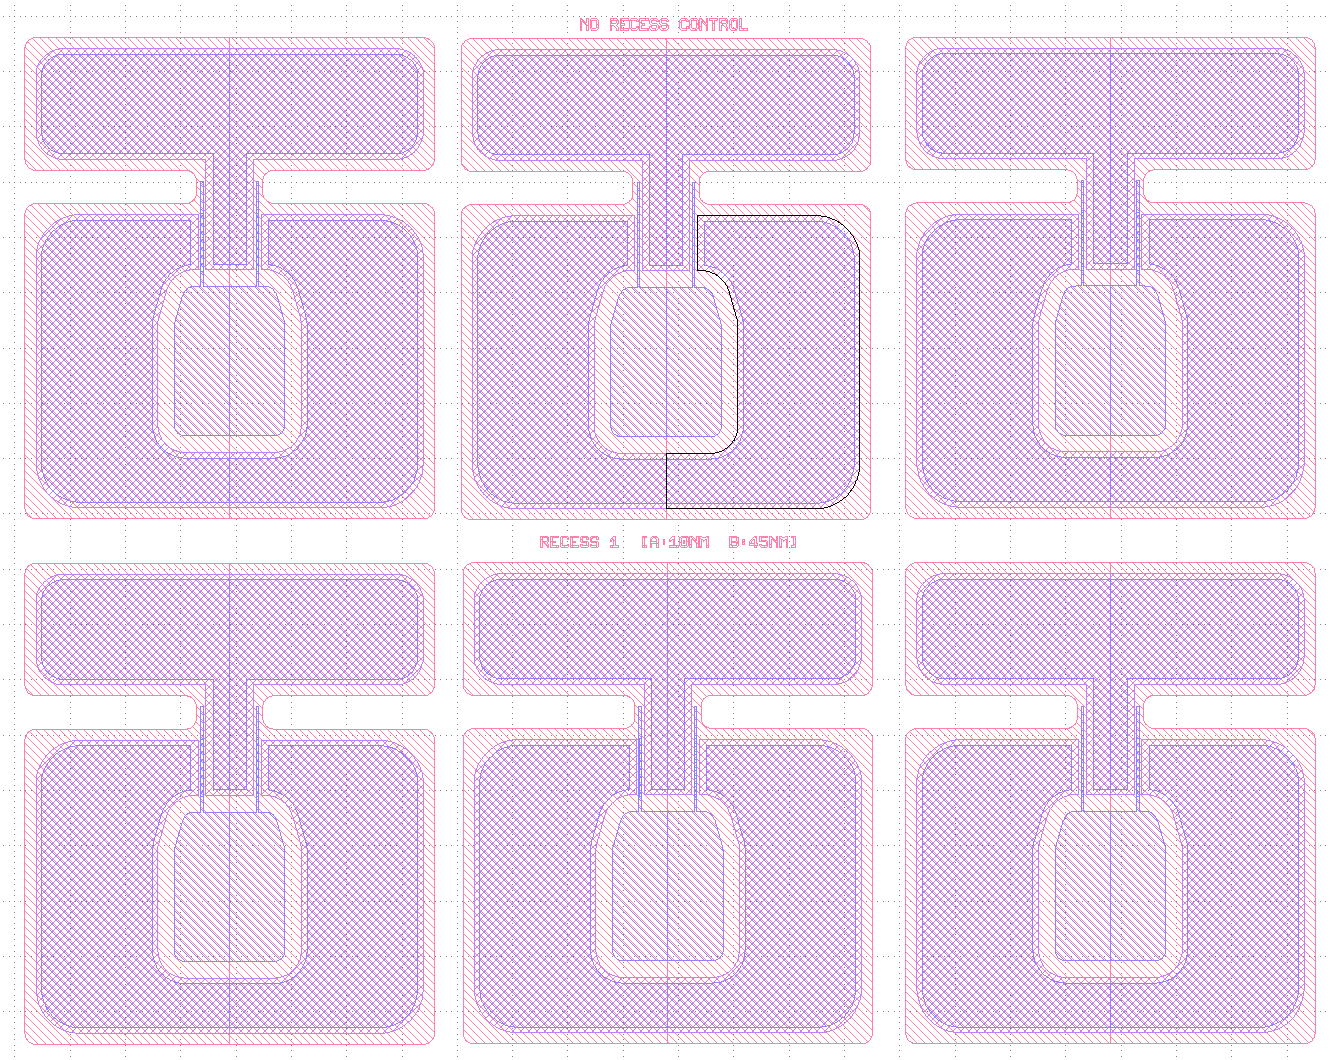
\includegraphics[width=12.3cm]{figures/gate_recession/quad_mask.png}
    };

    % Approximate control-device highlight: top row, second column.
    \coordinate (controlSW) at
      ($(quadmask.south west)!0.34!(quadmask.south east)
        +(0,0.40*12.3cm)$);
    \coordinate (controlNE) at
      ($(quadmask.south west)!0.66!(quadmask.south east)
        +(0,0.79*12.3cm)$);
    \draw[green!55!black, dashed, line width=2pt]
      (controlSW) rectangle (controlNE);
    \node[
      font=\small\bfseries,
      text=green!40!black,
      fill=white,
      fill opacity=0.75,
      text opacity=1,
      inner sep=1.5pt
    ] at ($(controlSW)!0.5!(controlNE)$) {Control Device};

    \begin{pgfonlayer}{background}
      \draw[red!75!black, dashed, line width=0.6pt]
        (zoomNW) -- (quadmask.north west);
      \draw[red!75!black, dashed, line width=0.6pt]
        (zoomNE) -- (quadmask.north east);
      \draw[red!75!black, dashed, line width=0.6pt]
        (zoomSW) -- (quadmask.south west);
    \end{pgfonlayer}

    \draw[red!75!black, dashed, line width=0.6pt]
      (zoomSE) -- (quadmask.south east);
  \end{tikzpicture}

  \vspace{2mm}
  \caption{Interleaved allocation of recess depths across two samples, with
  each quadrant containing the repeated set of five recessed devices and one
  unrecessed control device.}
  \label{fig:interleaved_quadrants}
  \label{fig:enhancement_mode_mask_quad}
\end{figure}


\FloatBarrier

\section{Structure of the Recessed Gate}

The gate recess does not only change the physical gate-to-channel separation;
it also changes the local band structure beneath the gate. Removing part of
the silicon-doped AlGaAs donor layer reduces the local donor supply to the
channel beneath the gate and raises the conduction-band edge in the recessed
region relative to the unrecessed regions, creating a local
conduction-band barrier. For the recessed device to conduct, the Schottky gate
must provide electrostatic control over the full recessed region so that an
applied positive gate bias can suppress this barrier sufficiently for carrier
transport through the channel.

\vspace{1mm}

This requirement affects the gate geometry. If the gate metal were deposited
only at the base of the trench, the centre of the recess would be modulated,
but the sidewall and recess-edge regions would remain weakly coupled to the
gate. These regions could retain residual conduction-band barriers, producing
non-uniform channel modulation and limiting current flow into the gated
region. The process was therefore designed so that the gate mask is wider
than the recess mask. This intentional lateral overlap allows the gate metal
to fill the trench and extend slightly onto the surrounding cap, producing a
T-shaped recessed-gate cross-section. The overlap improves electrostatic
coverage of the trench floor, sidewalls, and recess edges, and reduces
sensitivity to lithographic misalignment between the recess and gate layers.

\vspace{1mm}

Figure~\ref{fig:gate_overlap_electrostatics} illustrates this design
rationale. The band-edge sketches are qualitative rather than simulated band
diagrams. They show the intended physical interpretation: the unmetallised
recess in Figure~\ref{fig:gate_overlap_electrostatics}(a) introduces a local
barrier, incomplete gate coverage in
Figure~\ref{fig:gate_overlap_electrostatics}(b) lowers only the centre of the
barrier, and the overlapping T-gate in
Figure~\ref{fig:gate_overlap_electrostatics}(c) provides the most uniform
electrostatic control across the recessed region.

\vspace{5mm}

% figures/fig-gate-overlap-electrostatics.tex
% Gate overlap rationale for electrostatic control of a recessed gate.

\begin{figure}[htbp]
  \centering
  \resizebox{\linewidth}{!}{%
  \begin{tikzpicture}[x=0.82cm, y=0.58cm, >=Stealth, font=\scriptsize]

    \def\w{6.2}
    \def\hsub{0.75}
    \def\hchan{0.70}
    \def\hspacer{0.55}
    \def\hdonor{0.95}
    \def\hcap{0.45}
    \def\ytop{\hsub+\hchan+\hspacer+\hdonor+\hcap}
    \def\ydonorB{\hsub+\hchan+\hspacer}
    \def\ycapB{\hsub+\hchan+\hspacer+\hdonor}
    \def\xrecL{2.15}
    \def\xrecR{4.05}
    \def\yfloor{2.55}
    \def\panelGap{7.7}
    \def\bandY{-3.00}
    \def\bandH{1.35}
    \def\headerY{5.45}

    \path[use as bounding box] (-0.2,-5.05) rectangle (21.8,5.90);

    \newcommand{\drawrecessbase}[1]{%
      \begin{scope}[shift={(#1,0)}]
        \fill[gray!15] (0,0) rectangle (\w,\hsub);
        \fill[blue!8] (0,\hsub) rectangle (\w,\hsub+\hchan);
        \fill[green!8] (0,\hsub+\hchan) rectangle (\w,\hsub+\hchan+\hspacer);
        \fill[yellow!20]
          (0,\ydonorB) -- (\w,\ydonorB) -- (\w,\ycapB) --
          (\xrecR,\ycapB) -- (\xrecR,\yfloor) --
          (\xrecL,\yfloor) -- (\xrecL,\ycapB) --
          (0,\ycapB) -- cycle;
        \fill[red!15] (0,\ycapB) rectangle (\xrecL,\ytop);
        \fill[red!15] (\xrecR,\ycapB) rectangle (\w,\ytop);
        \draw (0,0) rectangle (\w,\hsub);
        \draw (0,\hsub) rectangle (\w,\hsub+\hchan);
        \draw (0,\hsub+\hchan) rectangle (\w,\hsub+\hchan+\hspacer);
        \draw
          (0,\ydonorB) -- (\w,\ydonorB) -- (\w,\ycapB) --
          (\xrecR,\ycapB) -- (\xrecR,\yfloor) --
          (\xrecL,\yfloor) -- (\xrecL,\ycapB) --
          (0,\ycapB) -- cycle;
        \draw (0,\ycapB) rectangle (\xrecL,\ytop);
        \draw (\xrecR,\ycapB) rectangle (\w,\ytop);
        \draw[blue,line width=0.75pt] (0,\hsub+\hchan) -- (\w,\hsub+\hchan);
      \end{scope}
    }

    \newcommand{\drawbandaxes}[1]{%
      \begin{scope}[shift={(#1,0)}]
        \draw[->, black!65] (0,\bandY) -- (\w+0.15,\bandY);
        \draw[->, black!65] (0,\bandY) -- (0,\bandY+\bandH+0.1);
        \node[anchor=east] at (-0.08,\bandY+\bandH) {$E_C$};
        \node[anchor=north] at (\w/2,\bandY-0.12) {position across recess};
      \end{scope}
    }

    % Column 1: unmetallised recess.
    \drawrecessbase{0}
    \begin{scope}[shift={(0,0)}]
      \node[font=\bfseries] at (\w/2,\headerY) {(a)};
      \drawbandaxes{0}
      \draw[red!70!black, line width=0.9pt, smooth]
        (0.15,\bandY+0.22) .. controls (1.70,\bandY+0.24) and (1.82,\bandY+1.22) ..
        (3.10,\bandY+1.25) .. controls (4.38,\bandY+1.22) and (4.50,\bandY+0.24) ..
        (6.05,\bandY+0.25);
    \end{scope}

    % Column 2: insufficient coverage.
    \drawrecessbase{\panelGap}
    \begin{scope}[shift={(\panelGap,0)}]
      \filldraw[fill=black!80, draw=black]
        (2.42,\yfloor) .. controls (2.70,\yfloor+0.62) and (3.50,\yfloor+0.66) ..
        (3.78,\yfloor) -- cycle;
      \node[anchor=south] at (3.10,\yfloor+0.58) {Gate};
      \node[font=\bfseries] at (\w/2,\headerY) {(b)};
      \drawbandaxes{0}
      \draw[red!70!black, line width=0.9pt, smooth]
        (0.15,\bandY+0.22) .. controls (1.50,\bandY+0.24) and (1.72,\bandY+1.18) ..
        (2.35,\bandY+1.12) .. controls (2.66,\bandY+0.42) and (3.54,\bandY+0.42) ..
        (3.85,\bandY+1.12) .. controls (4.48,\bandY+1.18) and (4.70,\bandY+0.24) ..
        (6.05,\bandY+0.25);
    \end{scope}

    % Column 3: overlapping T-gate.
    \drawrecessbase{2*\panelGap}
    \begin{scope}[shift={(2*\panelGap,0)}]
      \filldraw[fill=black!80, draw=black]
        (\xrecL-0.28,\ytop) -- (\xrecL-0.28,\ytop+0.42) --
        (\xrecR+0.28,\ytop+0.42) -- (\xrecR+0.28,\ytop) --
        (\xrecR,\ytop) -- (\xrecR,\yfloor) --
        (\xrecL,\yfloor) -- (\xrecL,\ytop) -- cycle;
      \node[anchor=south] at (\w/2,\ytop+0.42) {Gate};
      \node[font=\bfseries] at (\w/2,\headerY) {(c)};
      \drawbandaxes{0}
      \draw[red!70!black, line width=0.9pt, smooth]
        (0.15,\bandY+0.30) .. controls (1.55,\bandY+0.32) and (2.30,\bandY+0.34) ..
        (3.10,\bandY+0.32) .. controls (3.90,\bandY+0.34) and (4.65,\bandY+0.32) ..
        (6.05,\bandY+0.32);
    \end{scope}

  \end{tikzpicture}%
  }

  \caption{Recessed device cross-sections with qualitative band diagrams to demonstrate how gate 
  structure affects the electrostatics.}
  \label{fig:gate_overlap_electrostatics}
\end{figure}


\vspace{1mm}

The use of an overlapping gate was also a practical process requirement. A
self-aligned gate process was not used because gate
metallisation requires a bilayer resist stack to obtain the undercut profile
needed for lift-off. The recess and gate were therefore patterned in separate
lithography steps, making a perfect alignment with the recess trench incredibly challenging. 
Designing the gate to be wider than the trench provides the sufficient tolerance 
into the process while preserving the intended electrostatic function of 
the recessed gate.

\vspace{1mm}

\section{Etch Chemistry Selection and Calibration}

Several etching techniques can be used to implement the gate recess, most
notably dry plasma etching and wet chemical etching. Dry etching offers
superior depth control and repeatability \cite{Cadence2024}; however, it
also introduces increased process complexity and the risk of plasma-induced
surface damage, which can degrade the gate--semiconductor interface and
complicate interpretation of electrical results \cite{ZAPPE1993227}. For
this project, the priority was therefore not maximum depth precision alone,
but a low-damage, experimentally simple process with a sufficiently slow
etch rate that small timing errors would not dominate the intended
recess-depth variation.

\vspace{1mm}

For this reason, a wet chemical etch was selected. In particular, a dilute
sulphuric-acid-based solution was chosen to achieve relatively slow and
controllable etch rates, reducing the sensitivity of the process to timing
uncertainty. The selected chemistry was an H$_2$SO$_4$ : H$_2$O$_2$ :
H$_2$O mixture in the ratio 1 : 1 : 250, which is reported in the
literature to provide low etch rates in both GaAs and AlGaAs, making it
well suited to time-controlled recessing of the donor layer
\cite{guan_etching}.

\vspace{1mm}

To characterise the etch behaviour of this chemistry under the specific
conditions of this work, a calibration procedure was carried out in which
three independently processed samples were subjected to a structured sequence
of timed etch steps of increasing duration: 5\,s, 10\,s, 15\,s, 30\,s,
and 60\,s. The cumulative etch depth was measured by AlphaStep
profilometry after each interval. The resulting etch curves are presented in
Figure~\ref{fig:etch_calibration}(a). Rather than following a single
constant-rate trajectory, the untreated samples show a clear dependence on the
duration of each etch interval. Material removal is strongly suppressed for
the shortest steps, before increasing as the interval duration is
extended. This behaviour indicates that the apparent etch rate is not governed
only by the intrinsic GaAs or AlGaAs etch rate, but also by an additional
time-dependent process at the semiconductor surface.

% ------------------------------------------------------------
% File: figures/fig-etch-calibration.tex
% Wet-etch calibration plots without HCl pre-treatment.
% ------------------------------------------------------------

\begin{figure}[p]
  \centering
  \begin{subfigure}{0.99\linewidth}
    \centering
    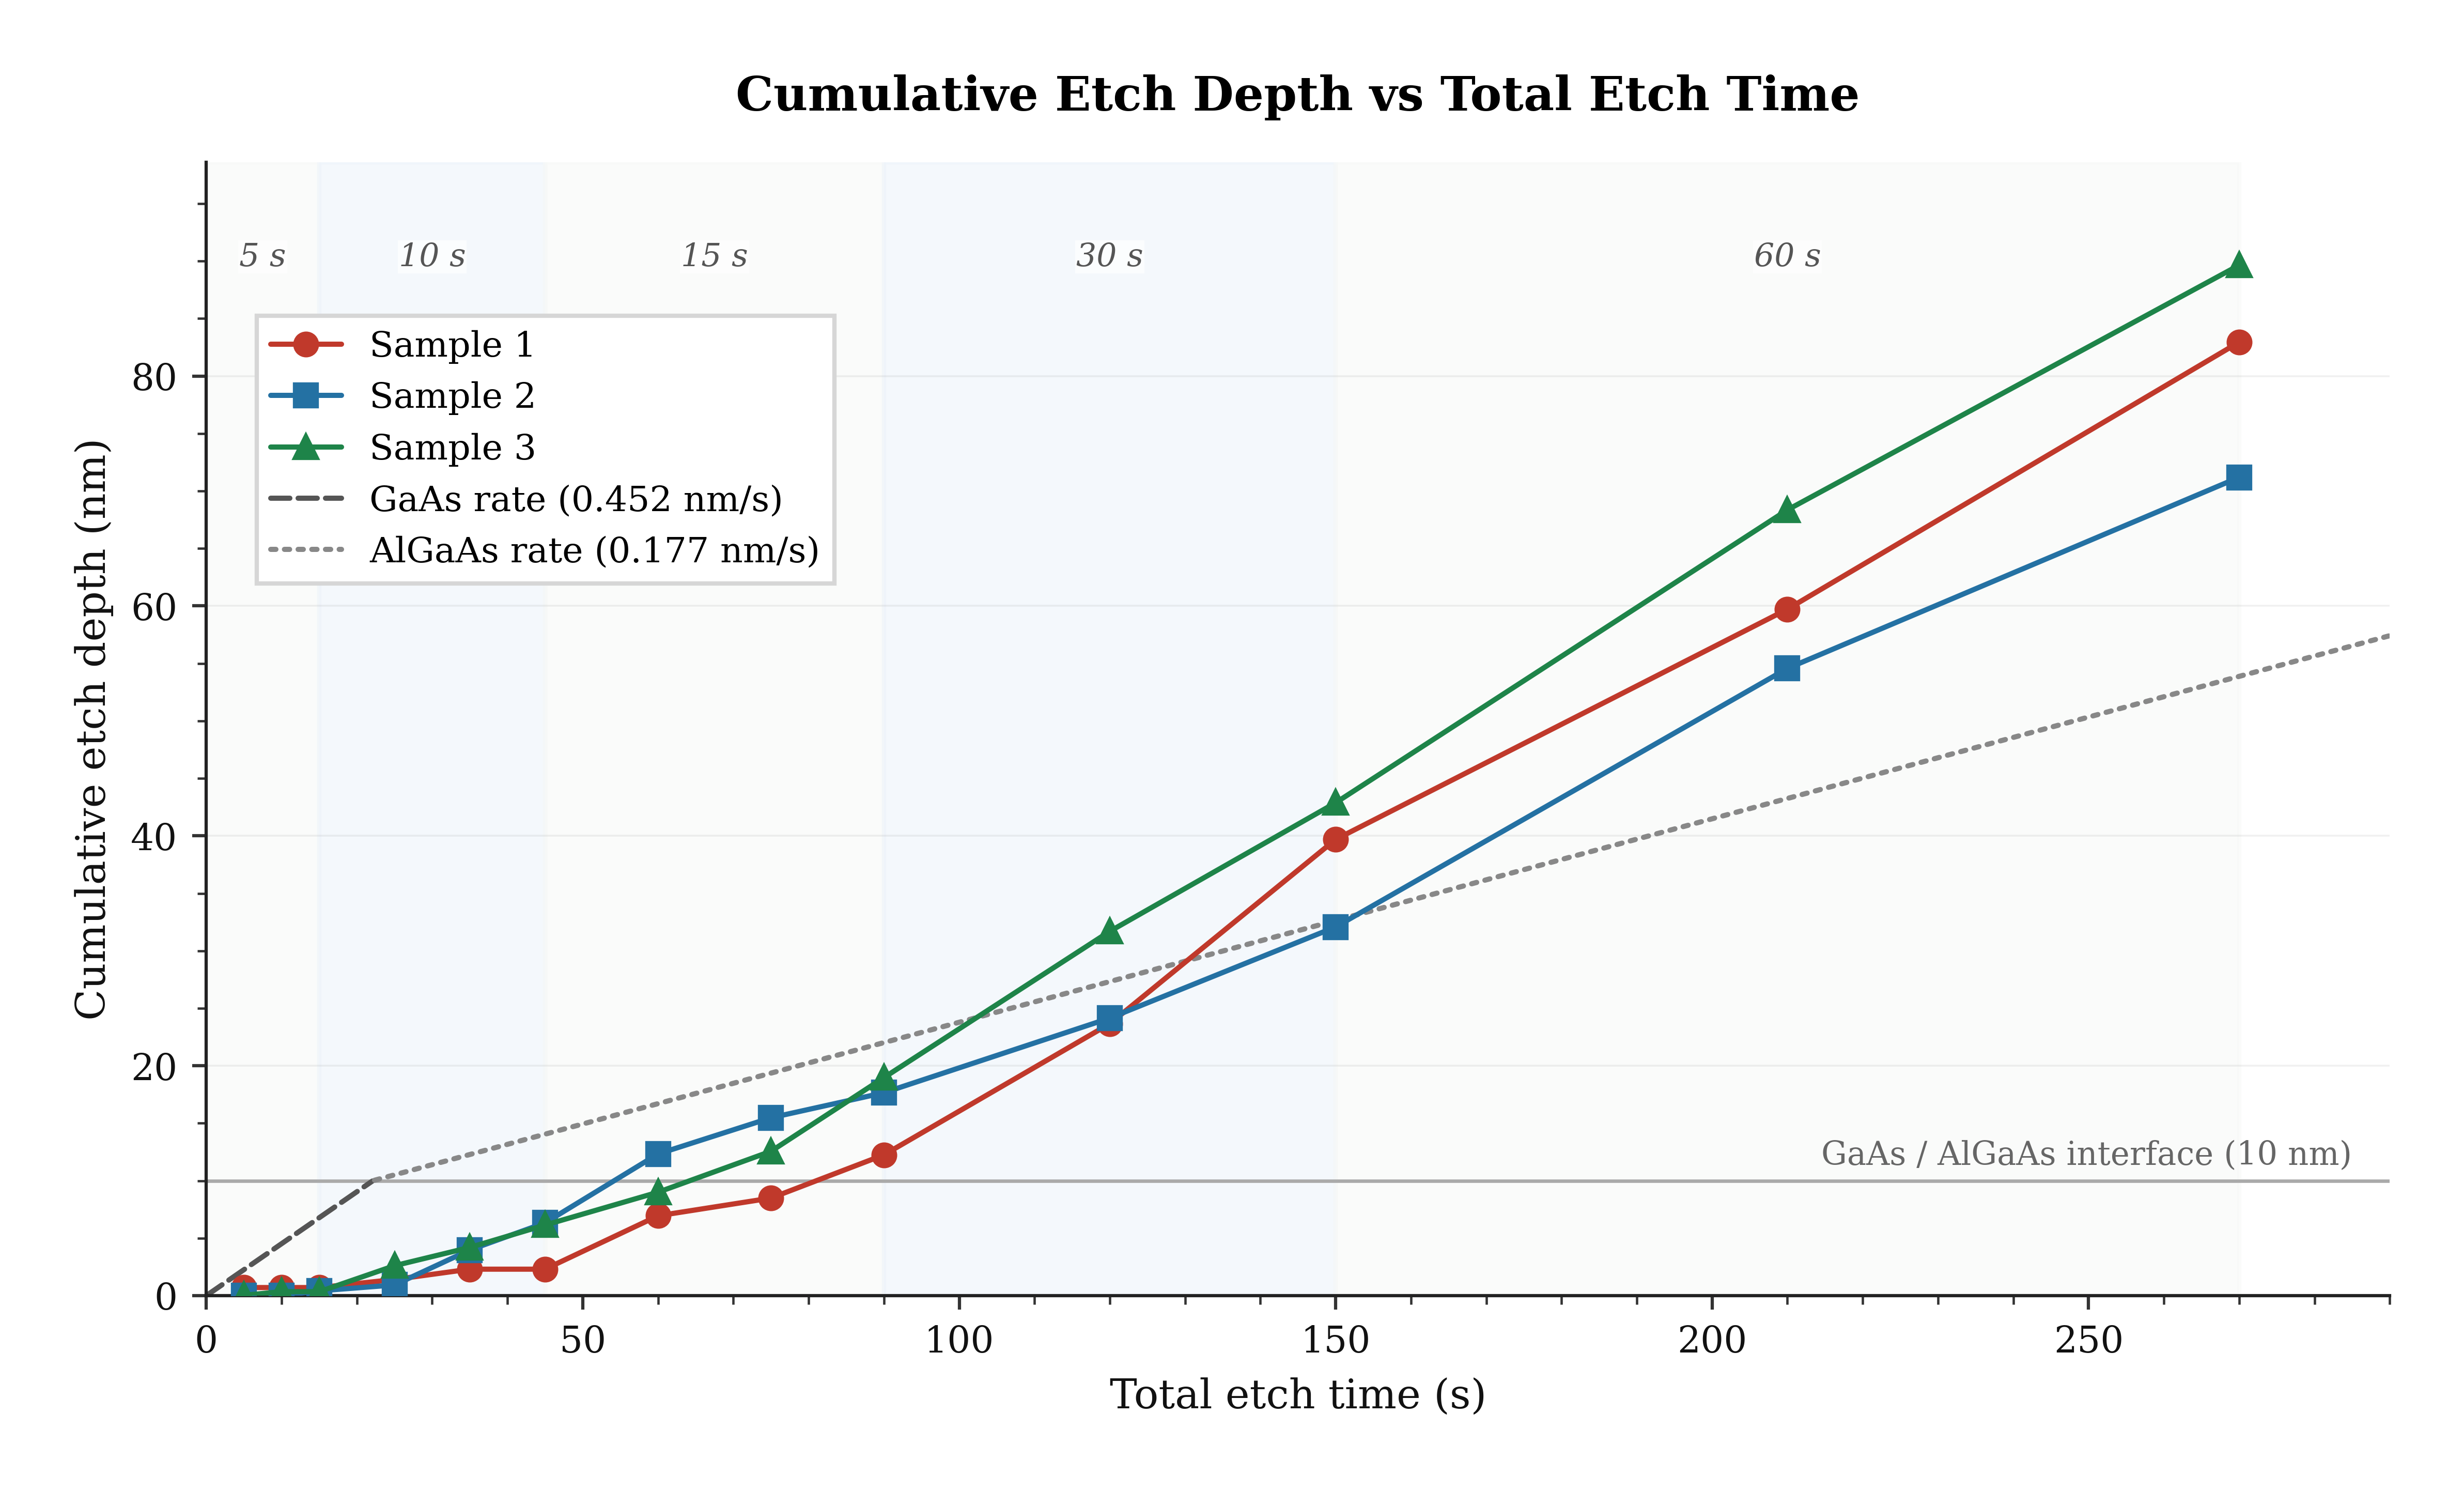
\includegraphics[width=\linewidth]{figures/electrical_analysis/etch_cumulative_depth.png}
    \caption{}
    \label{fig:etch_cumulative_depth}
  \end{subfigure}

  \vspace{-1mm}

  \begin{subfigure}{0.99\linewidth}
    \centering
    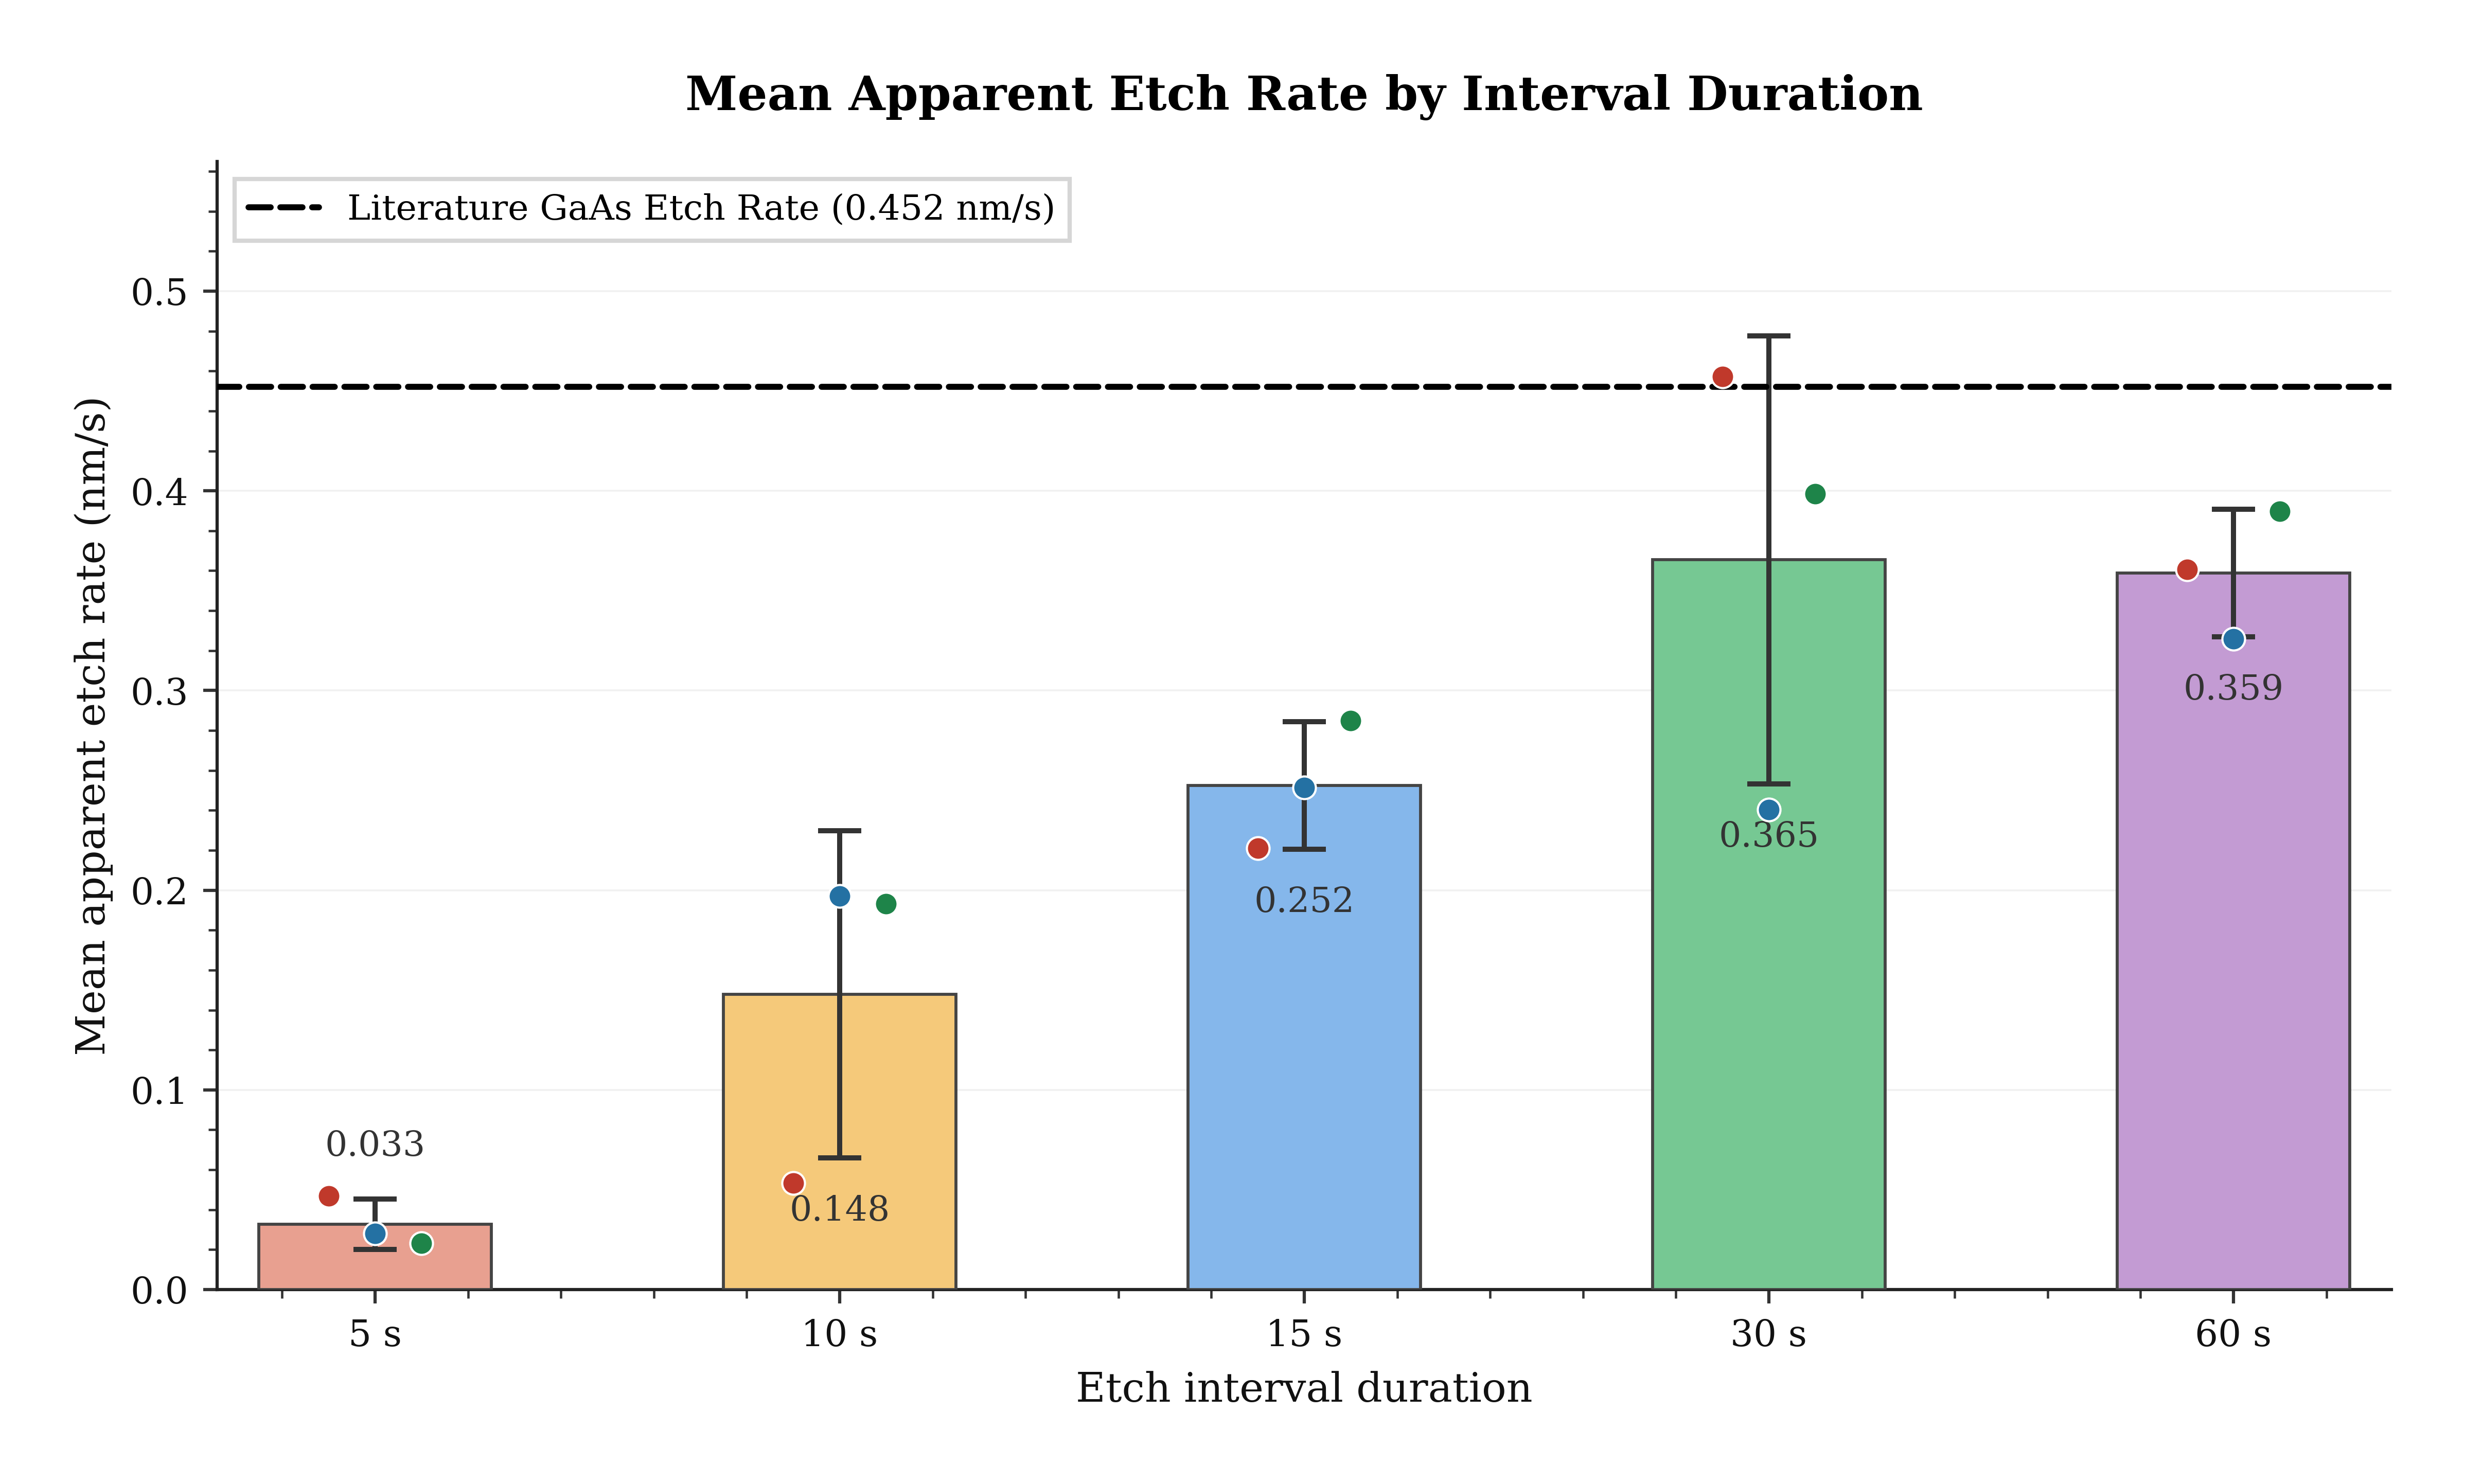
\includegraphics[width=\linewidth]{figures/electrical_analysis/etch_mean_apparent_rate.png}
    \caption{}
    \label{fig:etch_mean_apparent_rate}
  \end{subfigure}

  \caption{Wet-etch calibration without an HCl oxide-removal dip.}
  \label{fig:etch_calibration}
\end{figure}


This interval dependence is shown more directly in
Figure~\ref{fig:etch_calibration}(b), where the mean apparent etch rate is
defined as the mean depth increment per step divided by the interval duration.
The apparent rate rises with interval duration, from near zero at
5\,s to approximately $0.36\,\mathrm{nm\,s}^{-1}$ at 60\,s. Even at the
longest interval tested, the measured rate remains below the reported GaAs
rate of $0.452\,\mathrm{nm\,s}^{-1}$ for this chemistry \cite{guan_etching}.
This provides the key calibration result: the recess depth cannot be predicted
reliably from the nominal literature etch rate alone, particularly for the
short etch times relevant to shallow donor recessing.

\FloatBarrier

\section{Native Oxide Incubation and Mitigation}

The interval dependence is attributed to native oxide incubation. Each time a
sample is removed from solution for profilometry, the freshly etched GaAs or
AlGaAs surface is exposed to ambient air, allowing a native oxide layer of
approximately $2$--$3\,\mathrm{nm}$ to reform \cite{moriarty1992preliminary}.
At the start of the next H$_2$SO$_4$ : H$_2$O$_2$ : H$_2$O etch step, this
oxide must be dissolved before the underlying semiconductor is etched. The
oxide-removal period therefore consumes part of the timed interval without
producing a corresponding reduction in semiconductor thickness. This explains
why the 5\,s intervals produce negligible measured depth, why the 10\,s
intervals remain strongly suppressed, and why the apparent rate increases as
the etch interval becomes longer.

\vspace{1mm}

To test this hypothesis, a brief hydrochloric acid pre-dip
(HCl : H$_2$O = 1 : 5) was introduced immediately prior to each etch
interval on two additional samples, with the aim of chemically stripping the
native oxide before the sulphuric acid etch commenced. The effect on the
cumulative etch depth is shown in Figure~\ref{fig:hcl_etch_calibration}(a),
which compares the mean cumulative depth of the HCl-dipped samples ($n = 2$)
against that of the untreated samples ($n = 3$), with shaded bands indicating
the full inter-sample range in each case. The HCl-dipped samples display a
more linear cumulative-depth trajectory from the earliest intervals, while the
untreated samples retain the shallow initial response associated with oxide
incubation. The narrower shaded band for the HCl-dipped samples also indicates
improved uniformity between samples.

% ------------------------------------------------------------
% File: figures/fig-hcl-etch-calibration.tex
% HCl oxide-removal comparison for wet-etch calibration.
% ------------------------------------------------------------

\begin{figure}[p]
  \centering
  \begin{subfigure}{0.99\linewidth}
    \centering
    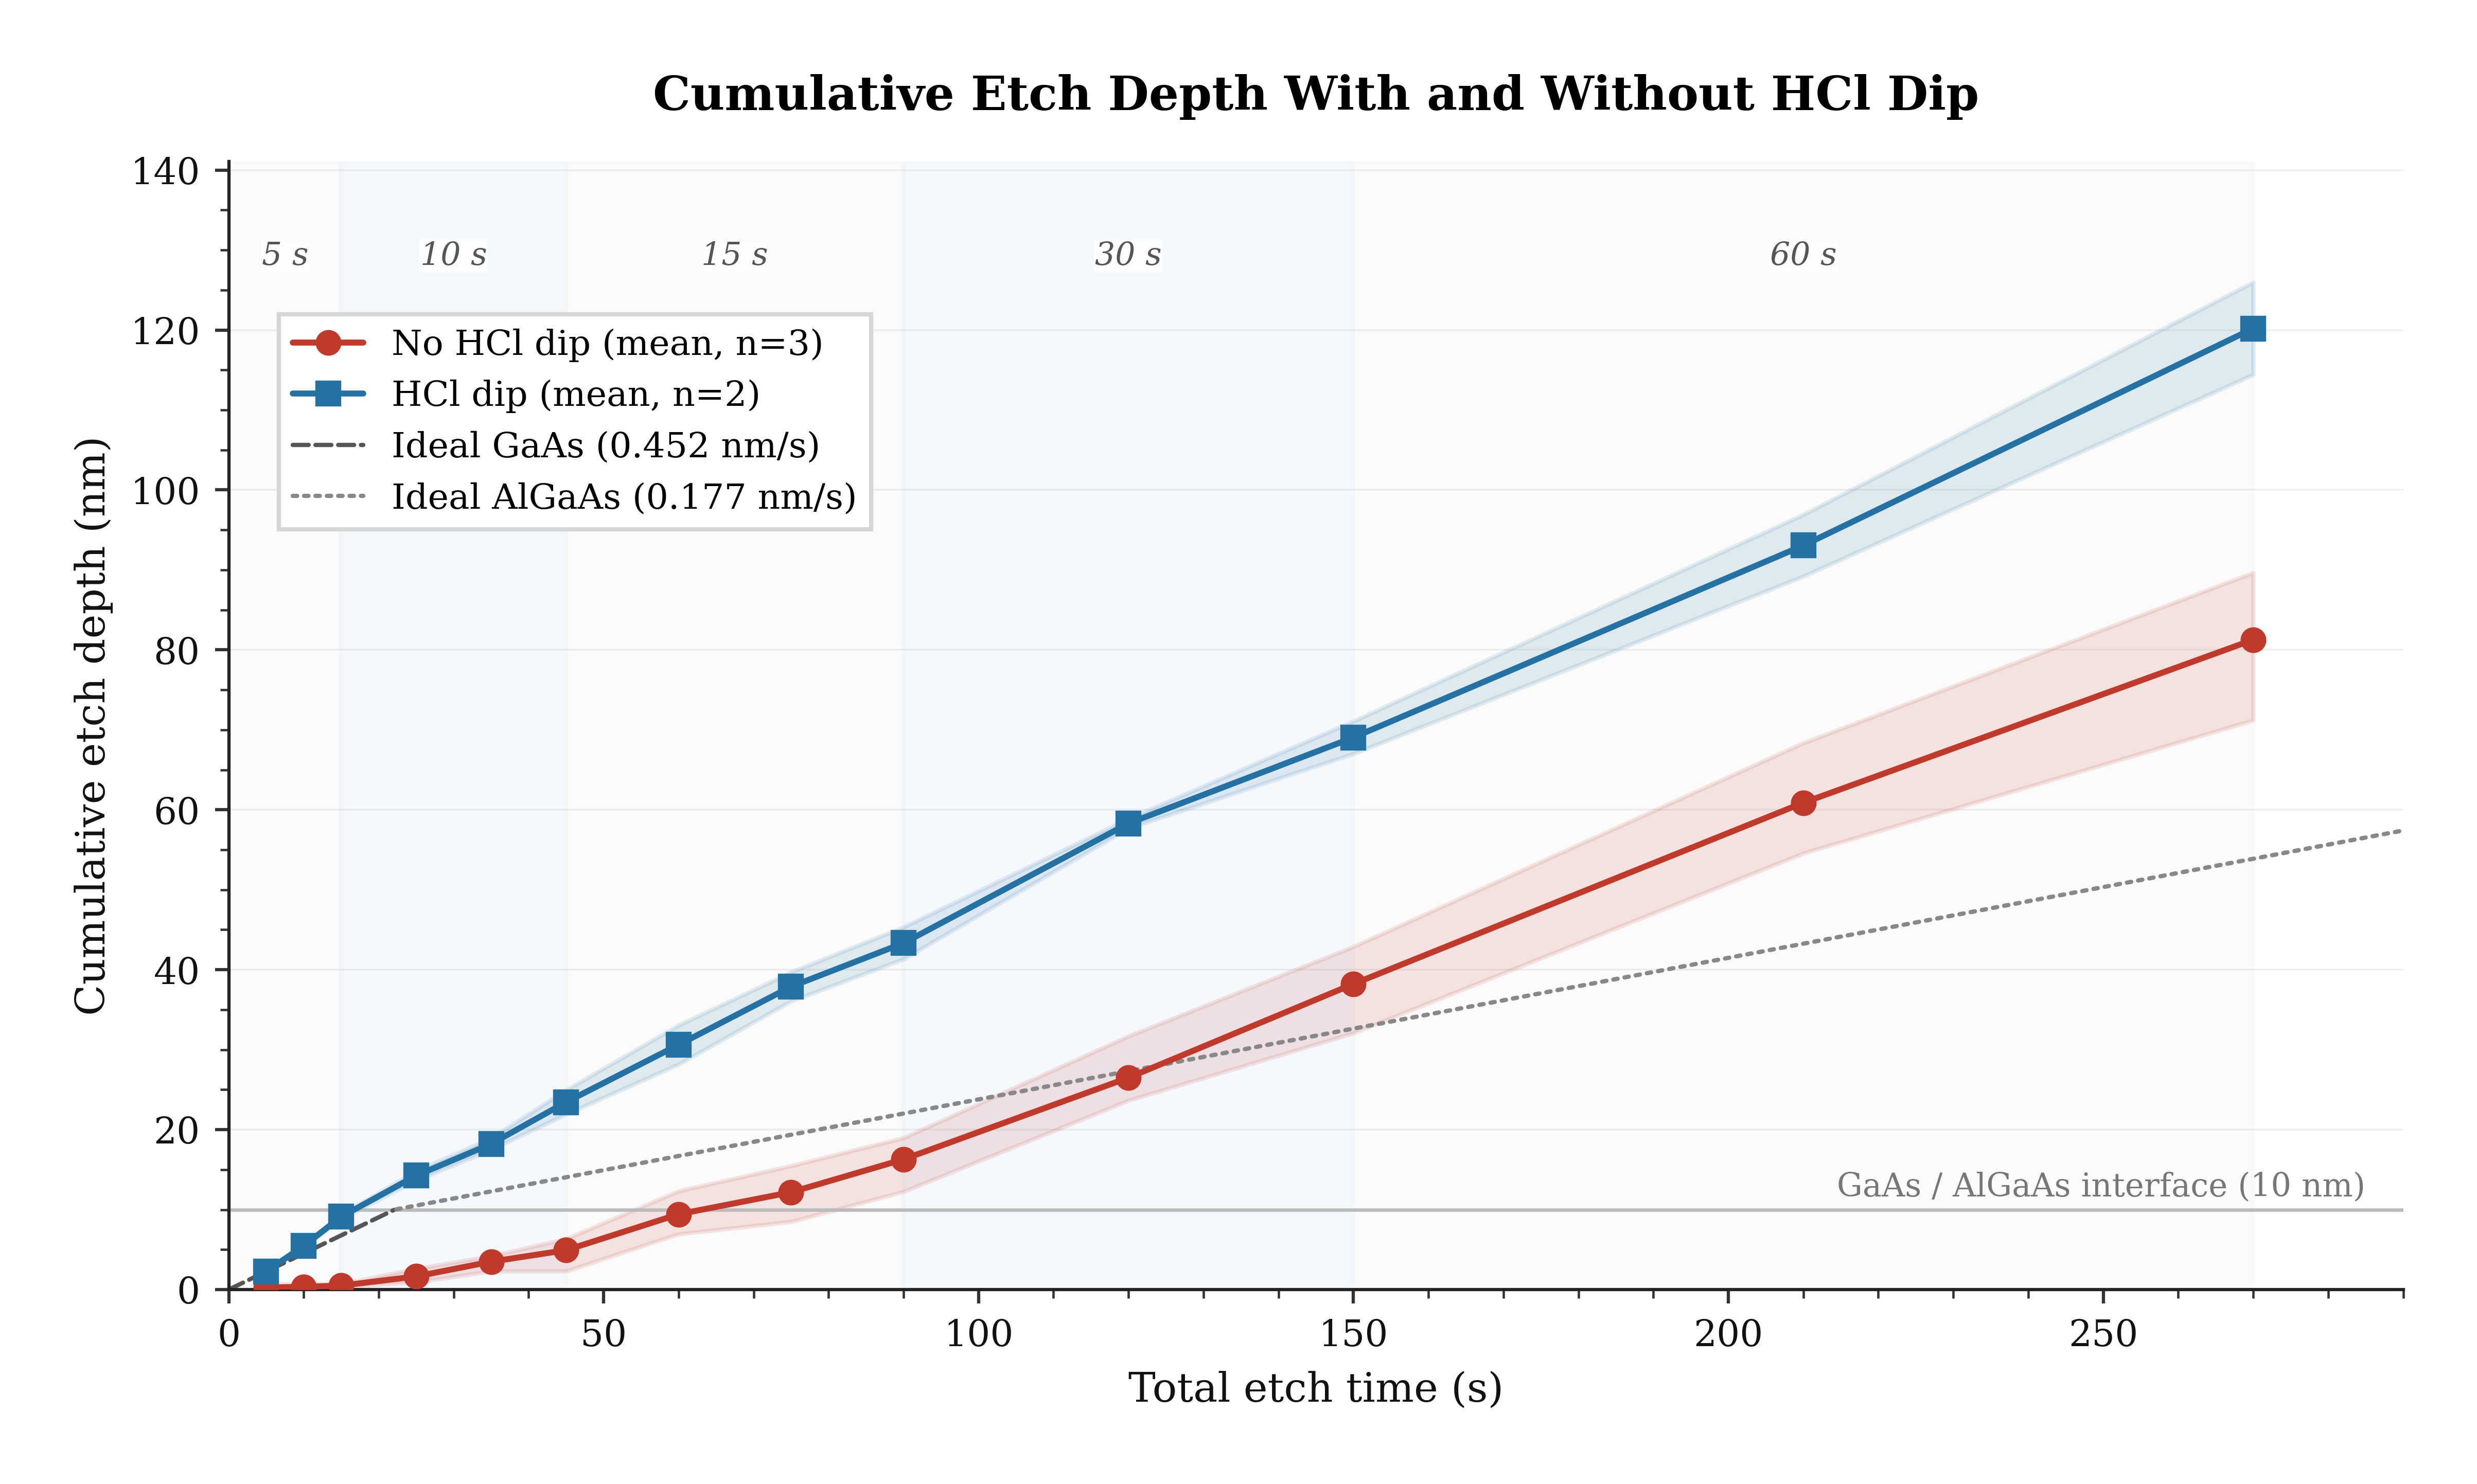
\includegraphics[width=\linewidth]{figures/electrical_analysis/etch_hcl_cumulative_depth.png}
    \caption{}
    \label{fig:etch_hcl_cumulative_depth}
  \end{subfigure}

  \vspace{-1mm}

  \begin{subfigure}{0.99\linewidth}
    \centering
    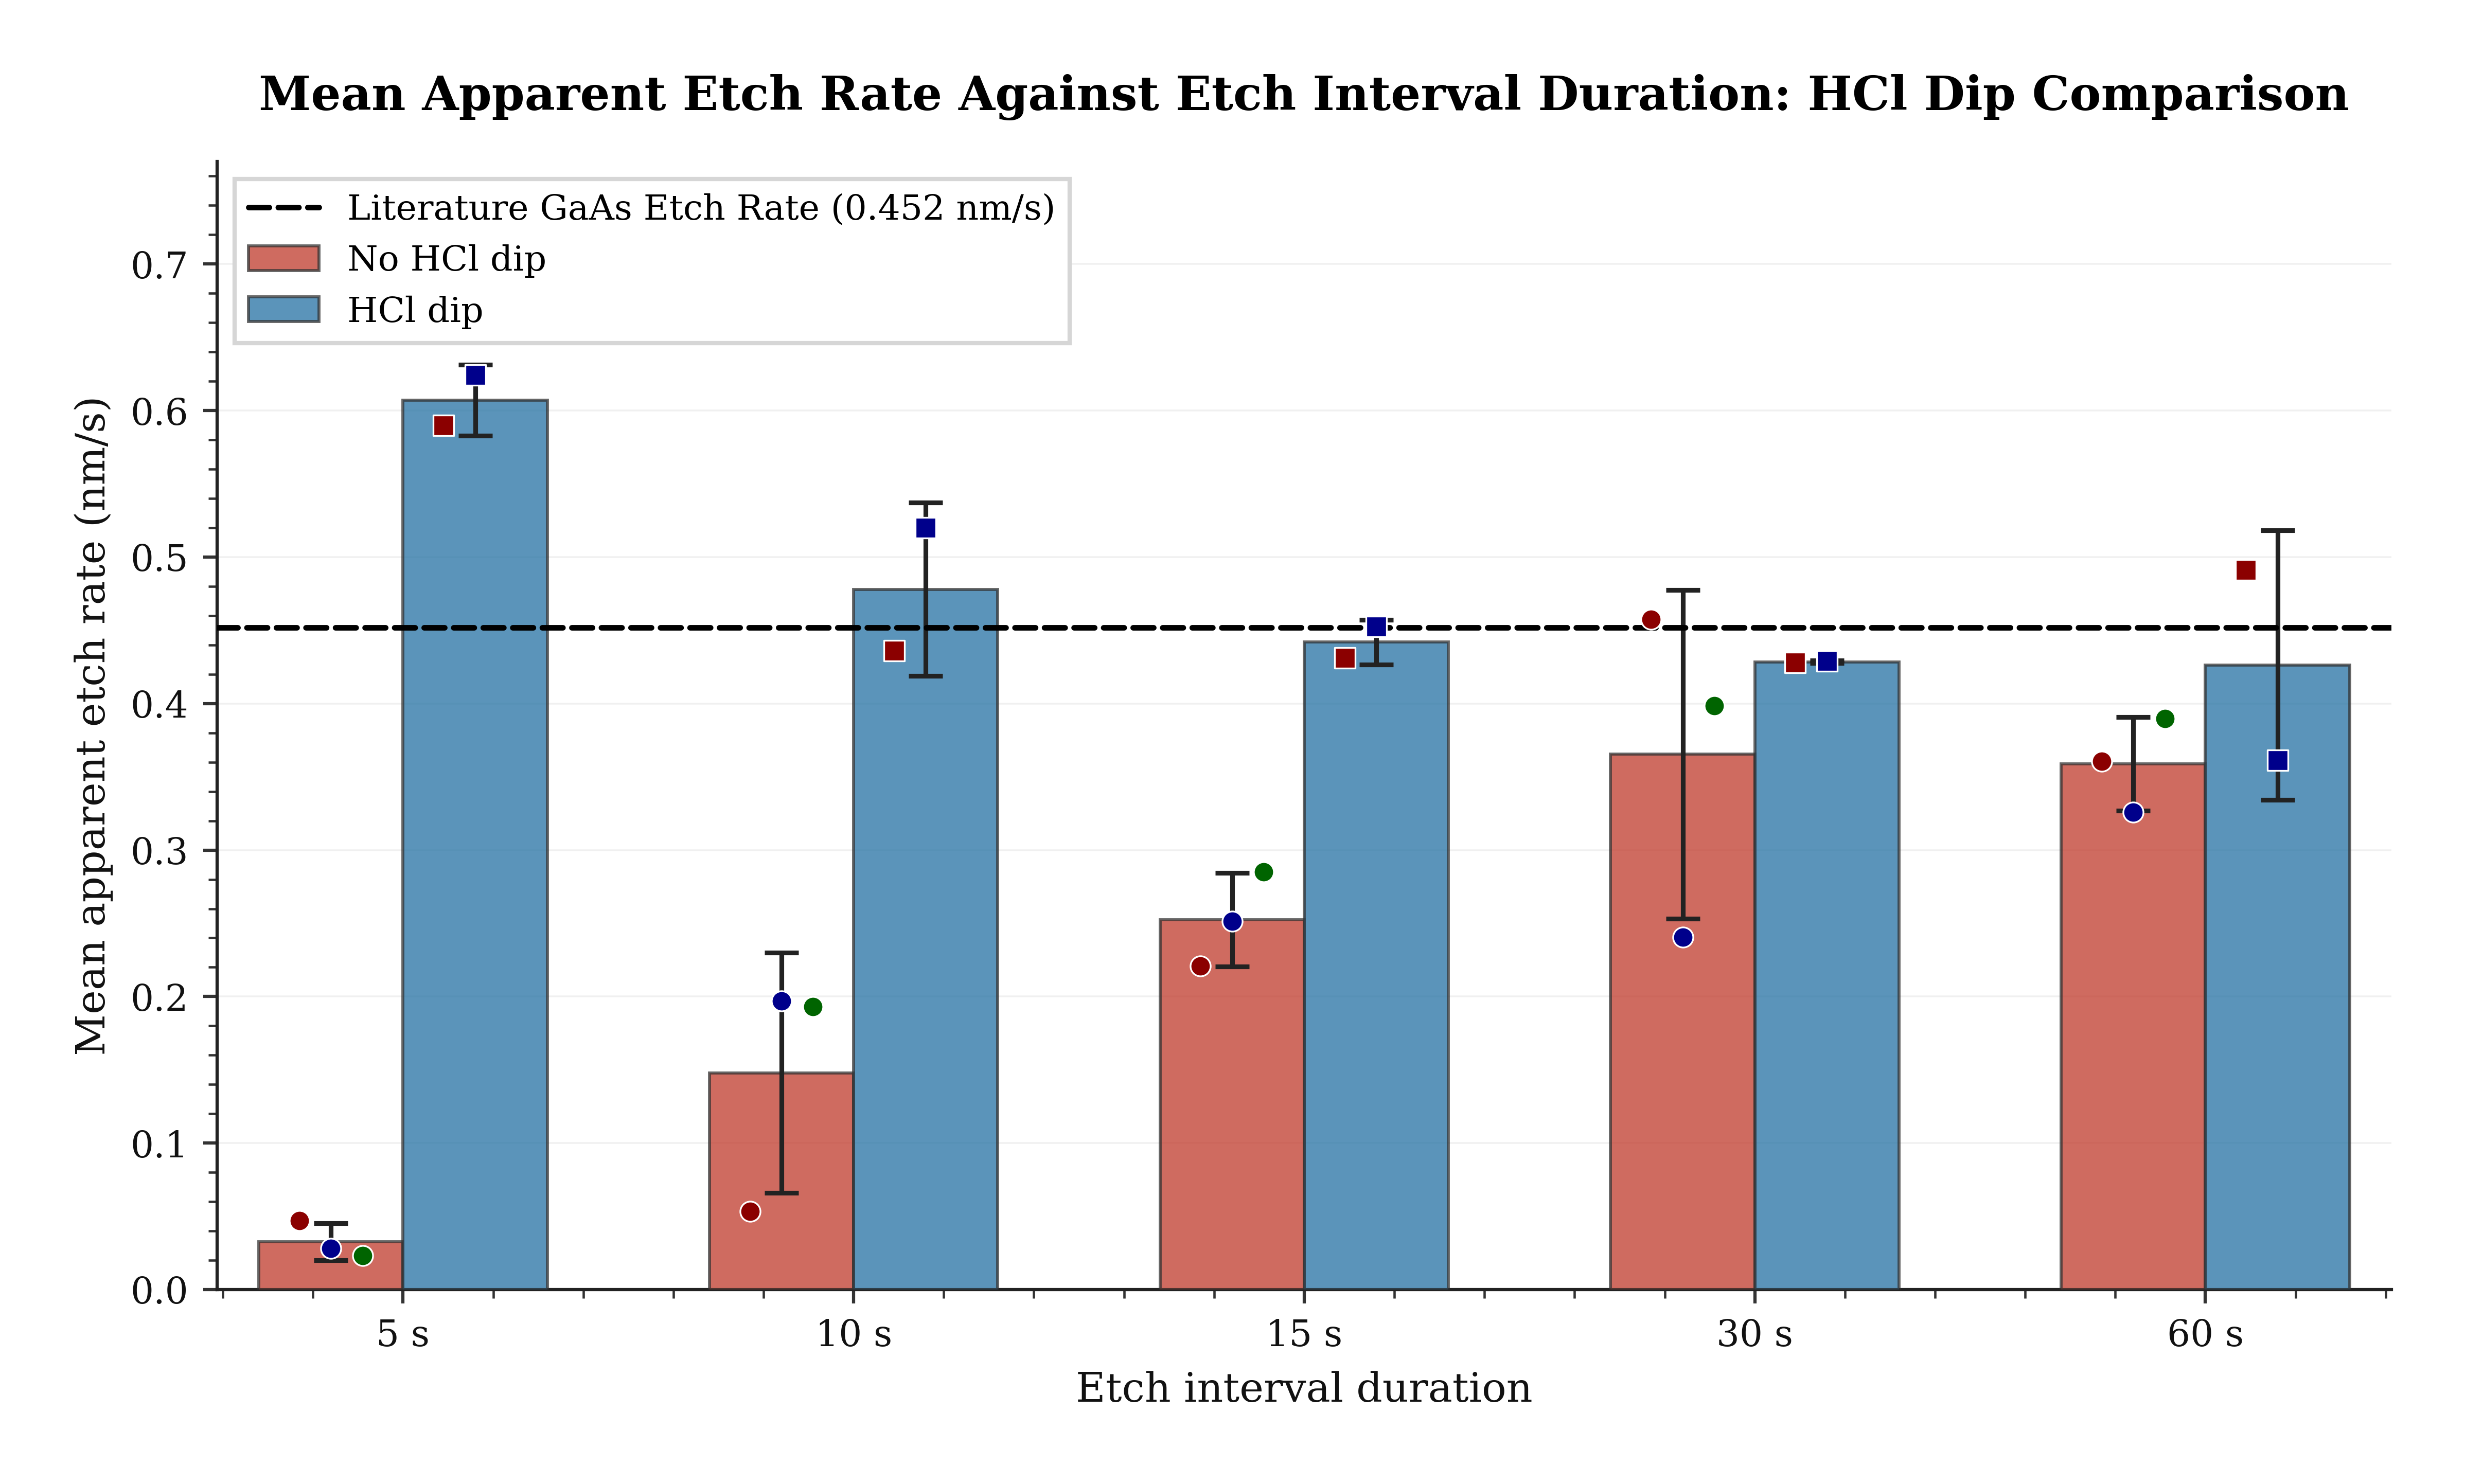
\includegraphics[width=\linewidth]{figures/electrical_analysis/etch_hcl_mean_apparent_rate.png}
    \caption{}
    \label{fig:etch_hcl_mean_apparent_rate}
  \end{subfigure}

  \caption{Wet-etch calibration comparison with and without the HCl
  oxide-removal dip.}
  \label{fig:hcl_etch_calibration}
\end{figure}


The corresponding apparent-rate comparison is presented in
Figure~\ref{fig:hcl_etch_calibration}(b). With the HCl pre-dip, the
apparent rate is much less dependent on the chosen interval duration and the
short-interval rates are substantially increased. The extracted rates approach
the reported GaAs value despite the etch extending into AlGaAs, whose wet etch
rate is normally reduced by oxide-mediated surface inhibition
\cite{guan_etching}. This is consistent with the combined effect of the HCl
pre-dip and agitation during etching: the HCl removes the native oxide before
the timed etch begins, while agitation helps prevent oxide or reaction-product
build-up at the surface and continually supplies fresh etchant to the recessed
region. Under these conditions, the effective AlGaAs etch behaviour becomes
closer to the GaAs rate than would be expected for a static, oxide-limited
etch.

Taken together, these results justify incorporating the HCl oxide-removal step
and controlled agitation into the gate recess process. The revised procedure
improves the linearity of depth with etch time and reduces the sample-to-sample
spread, both of which are essential for a depth sweep through a thin donor
layer. The calibrated process therefore provides a more reliable basis for
fabricating recessed-gate devices with deliberately varied threshold-voltage
targets.

\vspace{1mm}

\FloatBarrier
